\documentclass[%
a4paper,
twoside,
11pt
]{article} 

\usepackage{cookerybook}
\usepackage{blindtext}    % only needed for generating test text
\usepackage{hyperref}    % must be the last package
\usepackage{graphicx}



\hypersetup{%
	pdfauthor            = {Luca Lach, Robert Feldhans},
	pdftitle             = {Our Cookbook},
	pdfsubject           = {Recipes},
	pdfkeywords          = {recipes, cookbook, xcookybooky},
	pdfstartview         = {FitV},
	pdfview              = {FitH},
	pdfpagemode          = {UseNone}, % Options; UseNone, UseOutlines
	bookmarksopen        = {true},
	pdfpagetransition    = {Glitter},
	colorlinks           = {true},
	linkcolor            = {black},
	urlcolor             = {blue},
	citecolor            = {black},
	filecolor            = {black},
}

\hbadness=10000	% Ignore underfull boxes

\begin{document}
	
	\title{Our Cookbook}
	\author{Luca Lach\\ 
		\href{mailto:llach@techfak.uni-bielefeld.de}{llach@techfak.uni-bielefeld.de}\\
		Robert Feldhans\\ 
		\href{mailto:rfeldhans@techfak.uni-bielefeld.de}{rfeldhans@techfak.uni-bielefeld.de}}
	\maketitle
	
	\begin{abstract}
		Introduction to the cookbook.
	\end{abstract}
	
	
	\tableofcontents
	
	\section{Basics}
In this part of the book we will cover some basic knowledge and skills.

First we will discuss more general kitchen knowledge. %luca ergänz ma

In the second part, we will be focussing on food and its properties. That includes e.g. how to spot an ripe avocado, or what ingredients you could substitute with another. It should give you a more detailed view to one of the most crucial parts of cooking: The raw materials you use.

We will then take a look on the more science oriented side of things. Don't let the titel ``Chemistry'' fool you, a science degree won't be needed to understand this chapter. We will however take a look of the do's and dont's in regard to wanted -and unwanted- chemicl reactions that may occur in your kitchen.

In the end, we will then take a look at the first recipes. Those will not  provide you with a yummy and good meal, but they are for key components most other recipes rely on. We will for example see how onions are meant to be stewed and how noodles should be cooked.

\subsection{General Kitchen Knowlegde}

\subsubsection{How to get rid of fruit flies}

Who doesn't know and hate them: Fruit flies. Every year in the summer (and to some extend in the spring and fall to) they tend to swarm our kitchens and feast on our fruits. In case you don't want them to conquer your kitchen, here is a simple and cheap way to get rid of them:

What you will need:
\begin{itemize}
	\item a small bowl, maybe 10cm in diameter
	\item fruit juice, the sweeter the better. If you do not have any, or yours does not seem to wark, sugar is a good substitute
	\item water
	\item dish soap
\end{itemize}
You will want to fill the bowl with water and the juice (or sugar), so that the liquid is not too thick, it should be as close to water as possible. Then drop a bit of the dish soap into the bowl, stir for a bit and place it near your fruits, bio waste or whereever the most fruit flies seem to be. What will happen is that the fruit flies will try to drink the yummy sweet juice you gave them, but due to the absence of water stress the flies will not be able to walk on the water (what they normally could) and drown.

\subsection{Food Knowledge}

\subsection{Chemistry}

\subsection{Basic Ingredients}
	
	% Clearing pages depending on sided setting
	\if@twoside
		\cleardoublepage
	\else
		\clearpage 
	\fi
	
	\section{Recipes}
	who cleares the fucking page?! then again, we need a cover sheet for the recipes
	
	\timeFormat{100}\timeFormat{1}\timeFormat{60}
	
	% Test for new, clean recipe style
\begin{cleanrecipe}{Wraps con Carne}

	\g{500}{Rinderhack}
	\g{700}{Zwiebeln}
	
	\spicesg{300}{Pfeffer}
	\preparation{\blindtext}
\end{cleanrecipe}


	
\begin{center}
	\Huge 
	\textbf{Google Picture Search}\\
	\vspace*{-\baselineskip}
	\vspace{0.4cm}
	\rectangleplus{13cm}{0.04cm}{red}\\
	\normalsize
	\Oven
\end{center}
	\begin{wraptable}{l}{4cm}
		\begin{tabulary}{4cm}{rL}
			& \textbf{Zutaten} \\
			& \textbf{500g} Google \\
			& \textbf{4 EL} Bilder \\
			& \\
			& \textbf{Gewürze} \\
			& \textbf{32 TL} Suche \\
		\end{tabulary}
	\end{wraptable}	

\blindtext
\blindtext
\vfill
\begin{minipage}[b][0.5\textheight][t]{\textwidth}
		\centering
		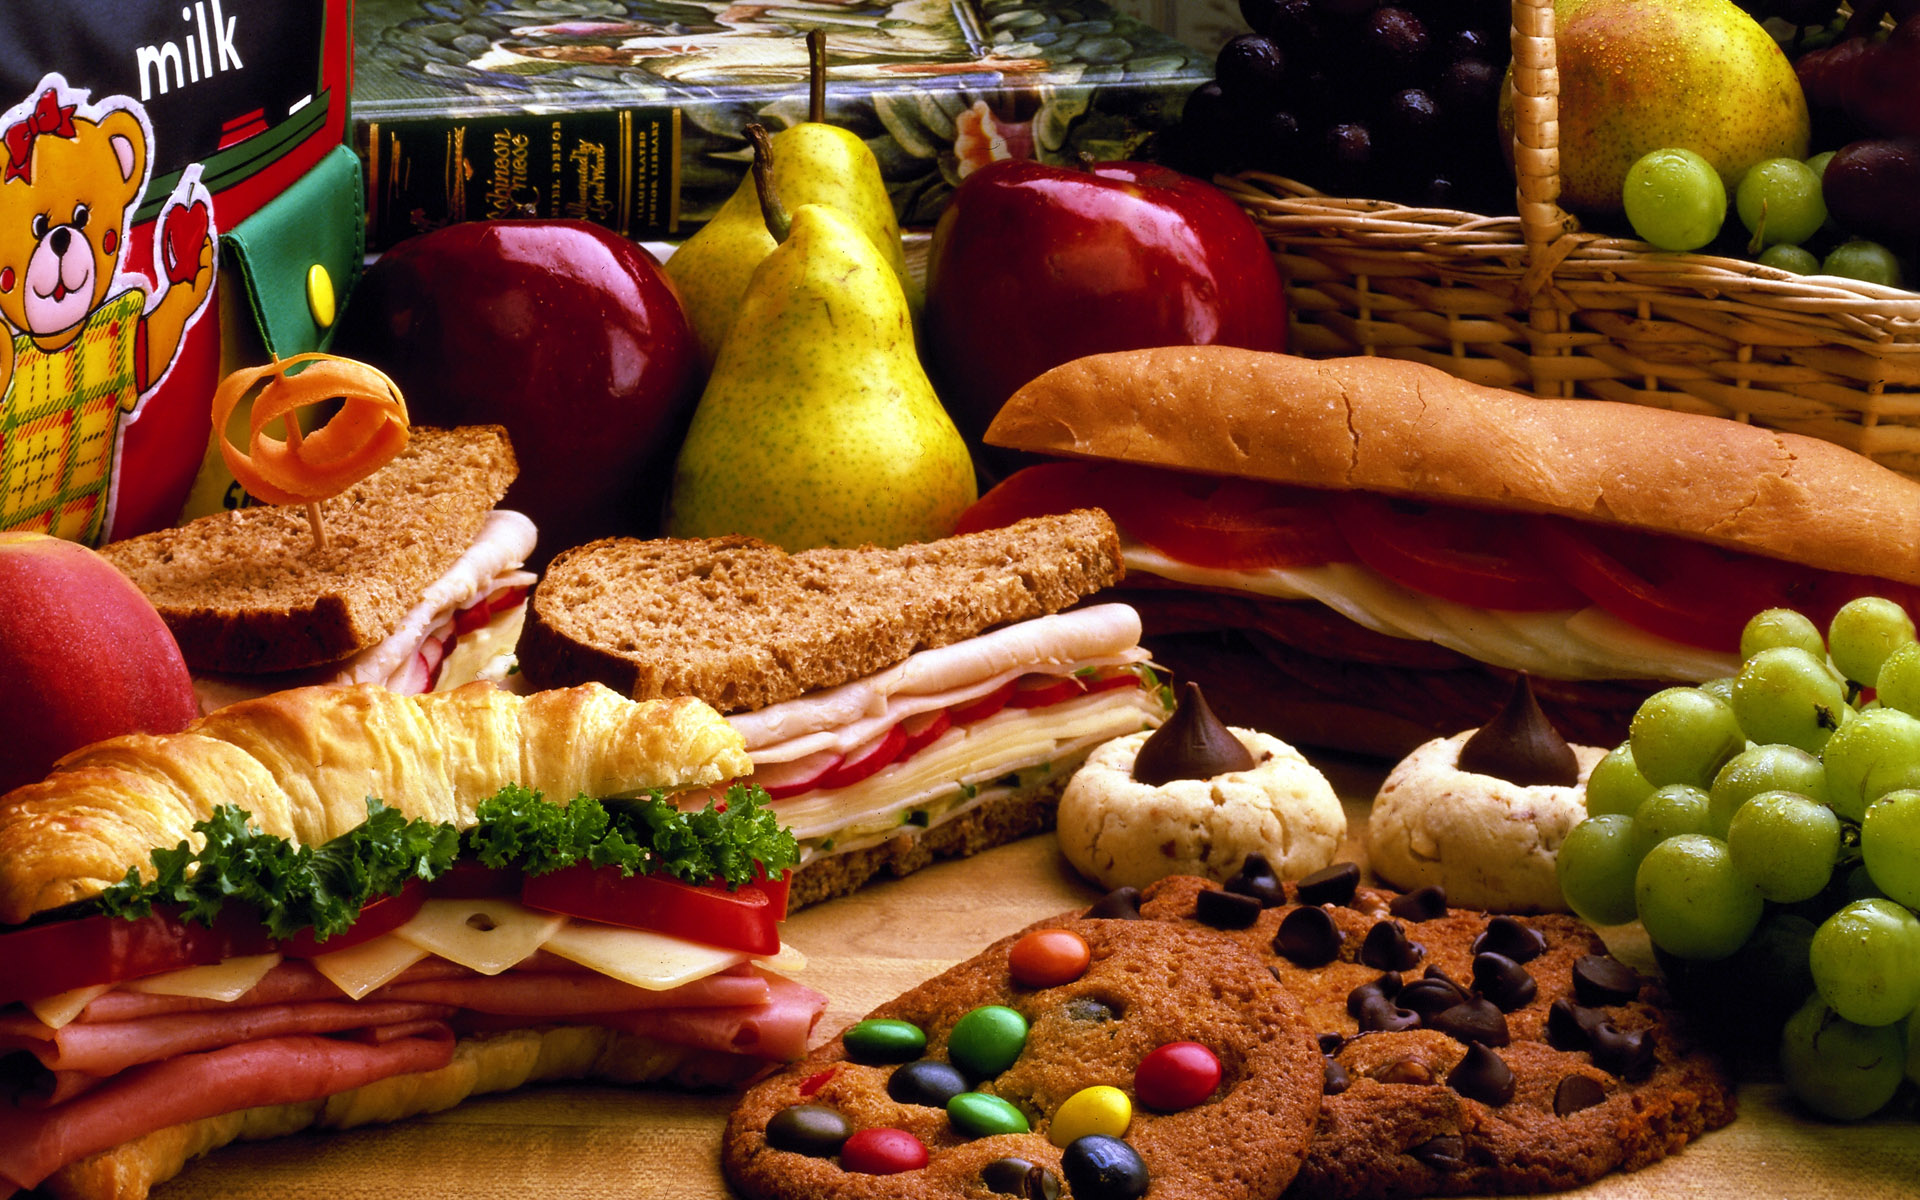
\includegraphics[width=\textwidth, height=0.35\textheight]{pictures/somefood.jpg}
\end{minipage}

\clearpage 

% Second recipe to test wheter the  variables are correctly handeled 
\begin{cleanrecipe}{Schrödingers Katze}
	\g{3}{Schödinger}
	\g{50}{Katze}
\end{cleanrecipe}

\iffalse
% Complete recipe example
\begin{recipe}
[% 
    preparationtime = {\unit[15]{min}},
    bakingtime={\unit[3-4]{h}},
    portion = {\portion{1}}
]
{Stired Onions}
    
    \graph
    {% pictures
    }
    
    \introduction{%
        Stired onions are actually really easy to make, even though they are often not done properly and many people are having trouble getting them right and not burning them. In this recipe, it will be almost impossible to burn them, they will be delicious, but on the downside it will take a really long time to make them.
    }
    
    \ingredients{%
        & Onions\\
        & Butter
    }
    
    \preparation{%
        \step Peel and cut the onions. The shape does not really matter, although you will mostly want little dice. For practise and some recipes, e.g. burgers, hoever you should use rings or half rings. The less thick the onios are cut, the less time this recipe will take. But make no mistake: As most of whats happening to the onions will take its time, no matter how thin the onions are sliced, it will always take quite long.
        
        \step Let the butter melt in a big pot. Seriously, you want a really big pot. A middle to big sized pan can also be used. Ideally the onions will just cover the bottom of the pot/pan. Most crucial in this will be the temperature. It should never be over 80\textcelcius, you will actually want it to be at around 60\textcelcius. The onions will at first not seem to change at all, and they shouldn't. But after about 3-4 hours, the onions will be perfect.
        
        \step Every now and then you will want to stir. This makes this recipe a bit tedious, as you are bound to the kitchen, and can only be away for so long. I would recommend stiring every 15 minutes. Depending on the type of pan or pot however this time will vary (a pan for example will lose more heat and thus will require more time to get the onions done but on the other hand you will get more time in between stirings).
        
        \step The onions are done when they are glassy and -depending on the type of onion- brownish-golden.
    }
    
    \hint{%
        Set alarms on your smartphone to not forget stirring.
    }
    
\end{recipe}
\fi
	
	
\end{document} 